% !TeX spellcheck = pt_BR
\documentclass[tese_patricia]{subfiles}
\begin{document}


\begin{comment}
	\nomenclature[F,01]{$\Omega_{x}$}{Domínio inicial de um sólido deformável;}

	
\end{comment}

% ---------------------------------------------------------- 
% Métodos de malhas sobrepostas
% ----------------------------------------------------------
\chapter[Método de Arlequin estabilizado]{Técnica de decomposição de domínios através do Método de Arlequin estabilizado - RBSAM} \label{capitulo:Cap6}
% ----------------------------------------------------------

Com intuito de superar os impasses encontrados com a técnica de decomposição de domínios apresentada no Cap. \ref{capitulo:Cap5}, neste capítulo será apresentado o método multiescala Arlequin.

A primeira parte deste capítulo será dedicada a descrever o método clássico de Arlequin, introduzido por \citeonline{Dhia:1998}. Na sequência, será apresentado o método de Arlequin estabilizado introduzido por \citeonline{FernandesEtAll:2020}  para a resolução de problemas de escoamento de fluidos incompressíveis. Por fim, será apresentada a descrição da técnica para problemas de contorno móveis e exemplos de validação serão exibidos.

\section{Método Arlequin}

O método Arlequin, introduzido por \citeonline{Dhia:1998}, consiste na superposição de um domínio local a um domínio global, em região efeitos localizados. Os modelos, local e global, são acoplados em uma zona de colagem através de operadores de Lagrange. 

O  método de Arlequin, de acordo com \citeonline{DhiaR:2005}, é baseado em três principais ideias ( ver Fig.\ref{DomLocalGlobal}):

\begin{itemize}
	\item Um domínio local $\localModel$ é sobreposto em um domínio global  $\globalModel$ em uma zona de interesse de modo a representar efeitos locais;
	\item Os modelos são colados um ao outro em uma subzona da zona de superposição ($\overlappingZone$) , chamada de zona de colagem ($\gluingZone$), através de um operador de acoplamento conveninente;
	\item  Garante-se a distribuição da energia entre os modelos empregando uma função ponderadora, definida a partir da partição da unidade;
\end{itemize}

\begin{figure}[htb!]
	\centering 
	%\vspace{-1em} % Diminui o espaço antes da figura
	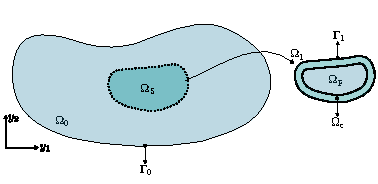
\includegraphics[scale=1.0,trim=0cm 0cm 0cm 0.0cm, clip=true]{Imagens/Cap6/dominioArlequin.pdf}	
	\caption{Domínio local e global}
	\label{fig:DomLocalGlobal}
	%\vspace{-1em} % Diminui o espaço antes da figura
\end{figure}

Dessa forma, o domínio computacional do problema é definido por:

\begin{align}
	\Omega = \globalModel + \localModel, \\
\end{align}

\noindent a zona de superposição, $\overlappingZone$, pode ser definida matematicamente da seguinte forma:

\begin{align}
	\overlappingZone = \globalModel \cap \localModel, \\
	\overlappingZone = \gluingZone \cup \freeZone, \\
	\overlappingZone > 0, \\
\end{align}

\noindent sendo  $\freeZone$ a chamada zona livre.

Umas das formas mais comuns de se realizar o acoplamento entre os modelos na zona de colagem $\gluingZone$ é através da aplicação de campos de multiplicadores de Lagrange. Uma forma generalizada de representar os operadores de acoplamento é apresentada em \citeonline{DhiaR:2002}, da maneira que se segue:

\begin{align}
	(\lagrangeMultiplier,\Delta u) =  \int_{\gluingZone} k_{0}[\lagrangeMultiplier \cdot \Delta u ] + k_{1}[\straintensor (\lagrangeMultiplier) : \straintensor (\Delta u)], \\
\end{align}

\noindent onde $\lagrangeMultiplier$ é o campo de multiplicadores de Lagrange, $\Delta u = \uglobal |_{\gluingZone} - \ulocal |_{\gluingZone}$ é a diferença entre os campos acoplados na zona de colagem. As constantes $k_{0}$ e $k_{1}$ são estritamente positivas. 

Quando $k_{0} > 0$ e $k_{1} = 0 $ têm-se o operador de acoplamento $L^{2}$. Esse acoplador estabelece a continuidade de ordem 0 do campo compatibilizado, que significada que ele garante no sentido de forma fraca, a continuidade das variáveis ao longo da zona de colagem. Para valores $k_{0} > 0$ e $k_{1} > 0 $ obtêm-se o operador de acoplamento $H_{1}$, que garante a continudade de ordem 1 ao campo compatibilizado, fazendo com que ele garanta no sentido de forma fraca, a continuidade de uma combinação de variáveis e seu Laplaciano \cite{GuidaultAndBelytschko2007}.

É importante mencionar que o sucesso do método, indiferente do tipo de operador adotado, depende da escolha apropriada dos parâmetros $k_{0}$ e $k_{1}$. Para o acoplamento utilizando $L^{2}$, devido a simplicidade da aplicação na restrição dos campos $\ulocal = \uglobal$ na zona de colagem, o condicionamento do sistema depende fortemente da adoção do parâmetro $k_{0}$. Por isso, esta é uma das razões que a maioria dos trabalhos realizados utilizando o método Arlequin aplica o operador $H_{1}$. Devido a dificuldade de encontrar parâmetros ótimos para o método, o trabalho de \citeonline{FernandesEtAll:2020} apresenta uma modificação na construção do operador de acoplamento $L^{2}$ que será apresentada adiante no texto.

A definição do espaço de funções para os operadores de Lagrange é muito importante. O método apresenta flexibilidade para usar uma discretização diferente da zona de colagem, entretanto, usualmente se adota um subconjunto do espaço de funções de um dos modelos sobrepostos.  

Por fim, para que o método não adicione energia ao sistema, é necessário que seja definida uma função ponderadora ($\arlequinWF$) que garanta a distribução da energia do sistema ao longo dos modelos sobrepostos. Em geral, essa função é definida, para cada um dos modelos da seguinte forma:

\begin{align}
\begin{cases} \arlequinWF_{i} \in [0;1] \ em \ \Omega, \\ \arlequinWFGlobal + \arlequinWFLocal = 1 \ em \ \Omega ,\\
\arlequinWF_{i} = 1 \ em \ \Omega_{i} \textbackslash \Omega_{j},  \ i \ \neq j, \\
\arlequinWF_{i}  = ka > 0 \ em \ \Omega_{f}, 
   \end{cases} \label{alphai}
\end{align}

\noindent com $i=0,1$ que varia em função do modelo em questão, e $ka$ uma constante arbitrariamente pequena para o método de Arlequin ser relevante \cite{Dhia:2008}, conforme pode ser observado na Fig. \ref{fig:constanteKa}. REVISAR ESSE TRECHO.


\begin{figure}[htb!]
	\centering 
	%\vspace{-1em} % Diminui o espaço antes da figura
	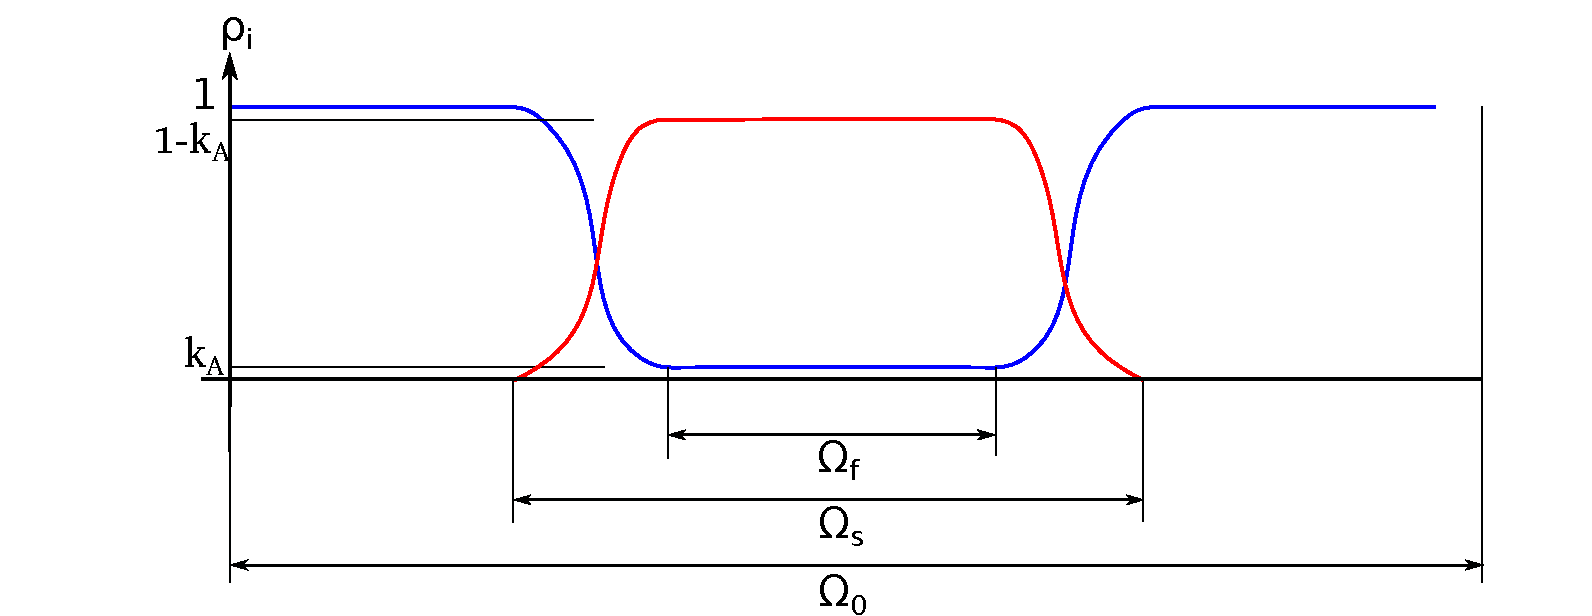
\includegraphics[scale=0.6,trim=0cm 0cm 1.5cm 0.0cm, clip=true]{Imagens/Cap6/ponderadora.pdf}	
	\caption{Função Ponderadora}
	\label{fig:constanteKa}
	%\vspace{-1em} % Diminui o espaço antes da figura
\end{figure}


\section{Método Arlequin clássico aplicado à problemas de escoamentos incompressíveis}

O método Arlequin vem sendo aplicado amplamente em diversos trabalhos da mecânica dos sólidos nas últimas décadas. Entretanto, no que diz respeito a materiais incompressíveis, pode-se citar mais recentemente o trabalho de \citeonline{JamondD:2013}, no qual os autores desenvolvem uma técnica para análise de sólidos incompressíveis empregando elementos do tipo Taylor-Hood, que satisfazem a condição LBB. Essa metodologia é testada também para problemas descritos pelas equações de Stokes.

De acordo com os autores \citeonline{JamondD:2013} a principal dificuldade encontrada para aplicação do método Arlequin no contexto de materiais incompressíveis é que duas restrições devem ser aplicadas concomitantemente: a compatibilização dos campos de interesse na zona de colagem e a condição de incompressibilidade do material nessa mesma região. Os autores apontaram que a imposição da condição de incompressibilidade em ambos os modelos pode gerar problema de redundância, acarretando em um sistema algébrico associado singular.

A solução proposta pelos autores nesse trabalho \cite{JamondD:2013} foi a aplicação da condição de incompressibilidade em cada ponto do domínio computacional apenas uma vez. A metodologia consiste então da remoção da condição de incompressibilidade dos elementos total ou parcialmente encontrados na zona de colagem ($\gluingZone$) em um dos modelos. Indiferente do modelo eleito para a remoção da condição de incompressibilidade na zona de colagem, na zona livre, a condição de incompressibilidade é removida do modelo global. Deve-se destacar que no trabalho citado existem algumas recomendações com relação a estabilidade da metodologiam, como por exemplo, a necessidade de existir pelo menos um elemento global na zona livre. Tal trabalho não explora as possíveis mudanças que acarretariam na estabilidade numérica em caso de sucessivas remoções e inclusões de condição de incompressibilidade no caso de um modelo local móvel.

Por esse motivo, e pelas pesquisas anteriores já realizadas pela presente autora e seu grupo de pesquisa, optou-se pela adoção de elementos estabilizados, os quais já foram retratos nos capítulos anteriores (Cap. \ref{capitulo:Cap2} e Cap. \ref{capitulo:Cap3}).

Para a construção do método de Arlequin clássico precisamos retomar às equações para um monomodelo apresentadas na seção \ref{capitulo:Cap2:FormaFraca} que representam a forma fraca discretizada espacialmente e estabilizada das equações da quantidade de movimento (Eq. \ref{eq:FinalSystem}) e da continuidade (Eq. \ref{eq:RC}). MUDAR AS EQUAÇÕES NO CAPÍTULO DE FLUIDOS PARA DEIXAR SEM O TERMO ALE INICIALMENTE.

Vamos considera os espaços de dimensão finita das funções tentativa que descrevem a velocidade ($\uArlequinSolution$) e a pressão ($\pArlequinSolution$) e os espaços de funções testes $\uArlequinTest$ e $\pArlequinTest$, com $i = 0,1$ indicando o índice do modelo, definidos como:

\begin{align}
	\uArlequinSolution = \left\{\velocity_{i}^{h} \left . \right| \velocity_{i}^{h} \left(\cdot,t\right) \in (H^{1h}\left(\Omega_{i}\right), \velocity_{i}^{h} = \velocity_{Di}^{h} \textrm { em}  \ \boundary_{Di} \right\}
\end{align}

\begin{align}
	\pArlequinSolution = \left\{\press_{i}^{h} \left . \right| \press_{i}^{h} \left(\cdot\right) \in L^{2h}\left(\domain_{i}\right) \right\},
\end{align}

\begin{align}
	\uArlequinTest = \left\{\utest_{i}^{h} \left . \right| \utest_{i}^{h} \left(\cdot\right) \in H^{1h}\left(\domain_i\right), \utest_{i}^{h} = \mathbf{0} \textrm { em} \ \boundary_{D_i} \right\},
\end{align}

e,

\begin{align}
	\pArlequinTest = \pArlequinSolution.
\end{align}

Analogamente, os espaços das funções tentativas ($\lagSolution$) e teste ($\lagTest$) para o campo dos multiplicadores de Lagrange ($\lagrangeMultiplier$) são definidos como:

\begin{align}
	\lagSolution = \left\{\lagrangeMultiplier^{h} \left . \right| \lagrangeMultiplier^{h} \left(\cdot\right) \in H^{1h}\left(\domain_{c}\right) \right\},
\end{align}

\begin{align}
	\lagTest = \lagSolution.
\end{align}

A aplicação do operador de acoplamento $L^{2}$ à formulação clássica Arlequin consiste em dado os espaços tentativa e teste apresentados nas equações anteriores: Encontrar $(\uglobalh,\pglobalh,\ulocalh,\plocalh,\lagrangeMultiplierh)$ $\in$ $\uGlobalSolution \times \pGlobalSolution \times \uLocalSolution \times \pLocalSolution \times \lagSolution$ de maneira que  $\forall$ $\wglobalh \in \uGlobalTest$, $\qglobalh \in \pGlobalTest$, $\wlocalh \in \uLocalTest$, $\qlocalh \in \pLocalTest$,   e $\forall$ $\lagrangeMultiplierWFh \in \lagTest$:

\begin{align}
	\begin{split}
		&\int_{\domain_0} \arlequinWFGlobal \density \wglobalh \cdot \frac{\partial\uglobalh}{\partial t} d\domain_{0} \\ 
		&\qquad+
		\int_{\domain_0} \arlequinWFGlobal \density \wglobalh \cdot  \left(\uglobalh \cdot \nabla\uglobalh\right) d\domain_{0}  \\ 
		&\qquad+	
		\int_{\domain_{0}} \arlequinWFGlobal \strainratetensor \left(\wglobalh\right) : \stresstensor \left(\uglobalh,\pglobalh\right)\ d\domain_{0} 
		 \\ 
		&\qquad+ \sum_{e=1}^{\nel} \int_{\domainE} \SUPG  \left(\left(\uglobalh \cdot \nabla \right) \wglobalh\right) \cdot \resMomGlobal\left(\uglobalh,\pglobalh \right)\  d\domain_{0} \\ 
		&\qquad+\sum_{e=1}^{\nel} \int_{\domainE} \LSIC \nabla \cdot \wglobalh \resPreGlobal 
		 \left(\uglobalh\right)\  d\domain_{0} \\
		 &\qquad+ \chi_{0} \int_{\domain_c} \wglobalh \cdot \lagrangeMultiplier^{h} d\domain_{c}  = \int_{\domain_0} \arlequinWFGlobal \density \wglobalh \cdot  \sbodyforce_{0}^{h} d\domain_{0} + \int_{\boundary_{0}} \arlequinWFGlobal \uglobalh \cdot \straction_{0}^{h}\ d\boundary_{0},
		\label{eq:FinalSystem0}
	\end{split}
\end{align}


\begin{align}
	\begin{split}
		&	\int_{\domain_{0}} \arlequinWFGlobal \qglobalh \nabla \cdot \uglobalh \ d\domain_{0} +
\sum_{e=1}^{\nel} \int_{\domainE} \PSPG \left(\frac{\nabla \qglobalh}{\density}\right) \cdot \resMomGlobal\left(\uglobalh,\pglobalh\right) \  d\domain_{0} = 0,
		\label{eq:RC0}
	\end{split}
\end{align}


\begin{align}
	\begin{split}
		&\int_{\domain_1} \arlequinWFLocal \density \wlocalh \cdot \frac{\partial\ulocalh}{\partial t} d\domain_{1} \\ 
		&\qquad+
		\int_{\domain_1} \arlequinWFLocal \density \wlocalh \cdot  \left(\ulocalh \cdot \nabla\ulocalh\right) d\domain_{1}  \\ 
		&\qquad+	
		\int_{\domain_{1}} \arlequinWFLocal \strainratetensor \left(\wlocalh\right) : \stresstensor \left(\ulocalh,\plocalh\right)\ d\domain_{1} 
		\\ 
		&\qquad+ \sum_{e=1}^{\nel} \int_{\domainE} \SUPG  \left( \right(\ulocalh \cdot \nabla \left) \wlocalh\right) \cdot \resMomLocal\left(\ulocalh,\plocalh \right)\  d\domain_{1} \\ 
		&\qquad+\sum_{e=1}^{\nel} \int_{\domainE} \LSIC \nabla \cdot \wlocalh \resPreLocal
		\left(\ulocalh\right)\  d\domain_{1} \\
		&\qquad+ \chi_{1} \int_{\domain_c} \wlocalh \cdot \lagrangeMultiplier^{h} d\domain_{c}  = \int_{\domain_1} \arlequinWFLocal \density \wlocalh \cdot  \sbodyforce_{1}^{h} d\domain_{1} + \int_{\boundary_{1}} \arlequinWFLocal \ulocalh \cdot \straction_{1}^{h}\ d\boundary_{1},
		\label{eq:FinalSystem1}
	\end{split}
\end{align}


\begin{align}
	\begin{split}
		&	\int_{\domain_{1}} \arlequinWFLocal \qlocalh \nabla \cdot \ulocalh \ d\domain_{1} +
		\sum_{e=1}^{\nel} \int_{\domainE} \PSPG \left(\frac{\nabla \qlocalh}{\density}\right) \cdot \resMomLocal \left(\ulocalh,\plocalh\right) \  d\domain_{1} = 0,
		\label{eq:RC1}
	\end{split}
\end{align}

\begin{align}
	\int_{\domain_{c}}  \lagrangeMultiplierWFh  \cdot \left(\uglobalh - \ulocalh \right) \ d\domain_{c} 
		\label{eq:EqAcopla}
\end{align}



\noindent onde $\resMomI$ e ${\resPreI}$ são os resíduos da equação da quantidade de movimento e da equação da continuidade, respectivamente, dados por:

\begin{align}
	\resMomI \left(\uArlqi,\pArlqi,\lagrangeMultiplierh \right)&=\arlequinWF_{i} \density\left(\frac{\partial\uArlqi}{\partial t}+ \left( \uArlqi \cdot \right) \nabla\uArlqi - \sbodyforce_i^{h}\right) - \arlequinWF_{i} \nabla \cdot \stresstensor\left(\uArlqi,\pArlqi\right)+ \chi_{i} \lagrangeMultiplierh \label{eq:resMomI},
\end{align}

\noindent

\begin{align}
	\resPreI\left(\uArlqi\right)&= \arlequinWF_{i} \nabla \cdot \uArlqi \label{eq:resPreI}, 
\end{align}

\noindent com $\chi_{i})$ descrito da maneira que se segue:


\begin{align}
	\chi_{i} = \begin{cases} (-1)^{i} \ se \ \mathbf{x} \in \domain_{c} \\
			   0 \ se \ \mathbf{x} \notin \domain_{c} \end{cases}.						. 
\end{align}

CONVERSAR COM O RODOLFO SOBRE ESSE TRECHO! 
O problema descrito pelas equações \ref{eq:FinalSystem0} à \ref{eq:EqAcopla} descreve à versão clássica do método de Arlequin para o problema de Navier-Stokes estabilizado pela técnica XXXXX. Matematicamente trata-se de um problema de ponto de sela decorrente de uma formulação mista. Entretanto, desde que a condição LBB seja satisfeita, existe solução para o problema e ela é única. 
Em \citeonline{GuidaultAndBelytschko2007} pode-se encontrar uma vasta análise matemática a cerca das questões relacionadas com estabilidade, convergência e relevância do método. Nesta pesquisa, os autores relatam, por exemplo, a necessidade de emprego de funções ponderadoras contínuas quando utilizado o operador de acoplamento $L^{2}$, tal caso não ocorre com o operador de acoplamento $H^{1}$. Além disso,  os autores destacam que espaçpos muito refinados para os acopladores de Lagrange podem levar a uma solução não convergente, independente do tipo de operador de acoplamento. Este problema ocorre devido a forte dependência da discretização do modelo global na solução.

O problema descrito no método Arlequin clássico é análogo a formução mista em elementos finitos para escoamentos incompressíveis, que limita a escolha das funções aproximadoras para o campo de velocidade e pressão. No caso da mecânica dos fluidos, conforme apresentado no Cap. \ref{capitulo:Cap2}, uma forma de superar esta restrição é o uso de métodos estabilizados como o PSPG. Seguindo essa mesma filosofia,  \citeonline{FernandesEtAll:2020} introduzem uma técnica de estabilização consistente que será apresentada na seguinte seção. 

\section{Método Arlequin estabilizado aplicado à problemas de escoamentos incompressíveis}


Com intuito de superar a condição LBB para o problema de Arlequin, \citeonline{FernandesEtAll:2020} desenvolvem uma técnica de estabilização consistente baseada em resíduo. Para isso, introduz-se uma parcela adicional à equação dos campos de multiplicadores de Lagrange, que leva em conta o gradiente de $\lagrangeMultiplierWFh$ e o resíduo da equação da quantidade de movimento:

\begin{align}
	\sum_{e=1}^{\nel} \int_{\domainE_{c}} \frac{\tauArlequinGlobal}{\rho} \nabla \lagrangeMultiplierWFh : \nabla \resMomGlobal \ d\domain_{c} - 
	\sum_{e=1}^{\nel} \int_{\domainE_{c}} \frac{\tauArlequinLocal}{\rho} \nabla \lagrangeMultiplierWFh : \nabla \resMomLocal \ d\domain_{c},
\end{align}

\noindent sendo $\tauArlequinGlobal$ e $\tauArlequinLocal$ parâmetros de estabilização, respectivamente da malha global e local, que devem ser suficientes para estabilizar o campo de multiplicadores de Lagrange sem comprometer a estabilidade do método. A obtenção destes parâmetros será abordada na subseção seguinte. 

Dessa forma, pode-se definir a solução do problema de Navier-Stokes para escoamentos incompressíveis utilizando a técnica de Arlequin estabilizada da seguinte forma: Encontrar $(\uglobalh,\pglobalh,\ulocalh,\plocalh,\lagrangeMultiplierh)$ $\in$ $\uGlobalSolution \times \pGlobalSolution \times \uLocalSolution \times \pLocalSolution \times \lagSolution$ de maneira que  $\forall$ $\wglobalh \in \uGlobalTest$, $\qglobalh \in \pGlobalTest$, $\wlocalh \in \uLocalTest$, $\qlocalh \in \pLocalTest$,   e $\forall$ $\lagrangeMultiplierWFh \in \lagTest$:

\begin{align}
	\begin{split}
		&\int_{\domain_0} \arlequinWFGlobal \density \wglobalh \cdot \frac{\partial\uglobalh}{\partial t} d\domain_{0} +
		\int_{\domain_0} \arlequinWFGlobal \density \wglobalh \cdot  \left(\uglobalh \cdot \nabla\uglobalh\right) d\domain_{0}  \\ 
		&\qquad+	
		\int_{\domain_{0}} \arlequinWFGlobal \strainratetensor \left(\wglobalh\right) : \stresstensor \left(\uglobalh,\pglobalh\right)\ d\domain_{0} 
		\\ 
		&\qquad+ \sum_{e=1}^{\nel} \int_{\domainE} \SUPG  \left(\left(\uglobalh \cdot \nabla \right) \wglobalh\right) \cdot \resMomGlobal\left(\uglobalh,\pglobalh \right)\  d\domain_{0} \\ 
		&\qquad+\sum_{e=1}^{\nel} \int_{\domainE} \LSIC \nabla \cdot \wglobalh \resPreGlobal 
		\left(\uglobalh\right)\  d\domain_{0} \\
		&\qquad+ \chi_{0} \int_{\domain_c} \wglobalh \cdot \lagrangeMultiplier^{h} d\domain_{c}  = \int_{\domain_0} \arlequinWFGlobal \density \wglobalh \cdot  \sbodyforce_{0}^{h} d\domain_{0} + \int_{\boundary_{0}} \arlequinWFGlobal \uglobalh \cdot \straction_{0}^{h}\ d\boundary_{0}, \\
		\label{eq:FinalSystem0est}
	\end{split}
\end{align}


\begin{align}
	\begin{split}
		&	\int_{\domain_{0}} \arlequinWFGlobal \qglobalh \nabla \cdot \uglobalh \ d\domain_{0} +
		\sum_{e=1}^{\nel} \int_{\domainE} \PSPG \left(\frac{\nabla \qglobalh}{\density}\right) \cdot \resMomGlobal\left(\uglobalh,\pglobalh\right) \  d\domain_{0} = 0, \\
		\label{eq:RC0est}
	\end{split}
\end{align}


\begin{align}
	\begin{split}
		&\int_{\domain_1} \arlequinWFLocal \density \wlocalh \cdot \frac{\partial\ulocalh}{\partial t} d\domain_{1} +
		\int_{\domain_1} \arlequinWFLocal \density \wlocalh \cdot  \left(\ulocalh \cdot \nabla\ulocalh\right) d\domain_{1}  \\ 
		&\qquad+	
		\int_{\domain_{1}} \arlequinWFLocal \strainratetensor \left(\wlocalh\right) : \stresstensor \left(\ulocalh,\plocalh\right)\ d\domain_{1} 
		\\ 
		&\qquad+ \sum_{e=1}^{\nel} \int_{\domainE} \SUPG  \left( \right(\ulocalh \cdot \nabla \left) \wlocalh\right) \cdot \resMomLocal\left(\ulocalh,\plocalh \right)\  d\domain_{1} \\ 
		&\qquad+\sum_{e=1}^{\nel} \int_{\domainE} \LSIC \nabla \cdot \wlocalh \resPreLocal
		\left(\ulocalh\right)\  d\domain_{1} \\
		&\qquad+ \chi_{1} \int_{\domain_c} \wlocalh \cdot \lagrangeMultiplier^{h} d\domain_{c}  = \int_{\domain_1} \arlequinWFLocal \density \wlocalh \cdot  \sbodyforce_{1}^{h} d\domain_{1} + \int_{\boundary_{1}} \arlequinWFLocal \ulocalh \cdot \straction_{1}^{h}\ d\boundary_{1}, \\
		\label{eq:FinalSystem1est}
	\end{split}
\end{align}


\begin{align}
	\begin{split}
		&	\int_{\domain_{1}} \arlequinWFLocal \qlocalh \nabla \cdot \ulocalh \ d\domain_{1}\\ +
		&\sum_{e=1}^{\nel} \int_{\domainE} \PSPG \left(\frac{\nabla \qlocalh}{\density}\right) \cdot \resMomLocal \left(\ulocalh,\plocalh\right) \  d\domain_{1} = 0, \\
		\label{eq:RC1est}
	\end{split}
\end{align}

\begin{align}
	\begin{split}
	&\int_{\domain_{c}}  \lagrangeMultiplierWFh  \cdot \left(\uglobalh - \ulocalh \right) \ d\domain_{c} + \sum_{e=1}^{\nel} \int_{\domainE_{c}} \frac{\tauArlequinGlobal}{\rho} \nabla \lagrangeMultiplierWFh : \nabla \resMomGlobal \ d\domain_{c} - \\
	&\sum_{e=1}^{\nel} \int_{\domainE_{c}} \frac{\tauArlequinLocal}{\rho} \nabla \lagrangeMultiplierWFh : \nabla \resMomLocal \ d\domain_{c},
	\label{eq:EqAcoplaest}
\end{split}
\end{align}

\noindent com os resíduos $\resMomI$ e $\resPreI$ escritos conforme as Eq. \ref{eq:resMomI} e Eq .\ref{eq:resPreI}.

O sistema resultante pode ser reescrito em notação matricial como:


\begin{align}
	\begin{bmatrix}
		\mathbf{K_{0}} & \mathbf{0} & \hat{\mathbf{L}_{0}} \\
		\mathbf{0} & \mathbf{K_{1}} & - \hat{\mathbf{L}_{1}} \\
		\mathbf{L}_{0}^{T} & -\mathbf{L}_{1}^{T} & \mathbf{E}
	\end{bmatrix}
	\begin{bmatrix}
		\mathbf{U_{0}} \\
		\mathbf{U_{1}} \\
		\mathbf{\lambda}
	\end{bmatrix}
	&=
	\begin{bmatrix}
		\mathbf{F_{0}} \\
		\mathbf{F_{1}} \\
		\mathbf{F_{\lambda}}
	\end{bmatrix}
	\label{eq:sistema_linear}
\end{align}	

Note que na estabilização Arlequin baseada no resíduo (RBSAM) não existem elementos zeros na diagonal da matriz, diferente do mesmo problema na formulação clássica Arlequin.

No trabalho de \citeonline{FernandesEtAll:2020} pode-se encontrar a análise de estabilidade dessa técnica e testes numéricos que avaliam o condicionamento do sistema algébrico e a convergência do método.

O problema de Arlequin não linear apresentado nas equações: Eq. \ref{eq:FinalSystem0est} à \ref{eq:EqAcoplaest} pode ser reescrito em sua forma semi-discreta residual para $i=0,1$, da seguinte maneira:

\begin{align}
	\begin{split}
		&\mathbf{R}_{M,i} = \int_{\domain_i} \arlequinWF_{i} \density \wArlqi \cdot \frac{\partial\uArlqi}{\partial t} d\domain_{i} +
		\int_{\domain_i} \arlequinWF_{i} \density \wArlqi \cdot  \left(\uArlqi \cdot \nabla\uArlqi\right) d\domain_{i}  \\ 
		&\qquad+	
		\int_{\domain_{i}} \arlequinWF_{i} \strainratetensor \left(\wArlqi\right) : \stresstensor \left(\uArlqi,\pArlqi\right)\ d\domain_{i} 
		\\ 
		&\qquad+ \sum_{e=1}^{\nel} \int_{\domainE} \SUPG  \left( \right(\uArlqi \cdot \nabla \left) \wArlqi\right) \cdot \resMomI \left(\uArlqi,\pArlqi \right)\  d\domain_{i} \\ 
		&\qquad+\sum_{e=1}^{\nel} \int_{\domainE} \LSIC \nabla \cdot \wArlqi \resPreI
		\left(\uArlqi\right)\  d\domain_{i} \\
		&\qquad+ \chi_{i} \int_{\domain_c} \wArlqi \cdot \lagrangeMultiplier^{h} d\domain_{c} - \int_{\domain_i} \arlequinWF_{i} \density \wArlqi \cdot  \sbodyforce_{i}^{h} d\domain_{i} - \int_{\boundary_{i}} \arlequinWF_{i} \uArlqi \cdot \straction_{i}^{h}\ d\boundary_{i},
		\label{eq:ResidualMomentum}
	\end{split}
\end{align}


\begin{align}
	\begin{split}
		&\mathbf{R}_{C,i} = \int_{\domain_{i}} \arlequinWF_{i} \qArlqi \nabla \cdot \uArlqi \ d\domain_{i} +
		\sum_{e=1}^{\nel} \int_{\domainE} \PSPG \left(\frac{\nabla \qArlqi }{\density}\right) \cdot \resMomI \left(\uArlqi,\pArlqi \right) \  d\domain_{i} = 0,
		\label{eq:ResidualContinum}
	\end{split}
\end{align}

\begin{align}
	\begin{split}
		&\mathbf{R}_{L} = \int_{\domain_{c}}  \lagrangeMultiplierWFh  \cdot \left(\uglobalh - \ulocalh \right) \ d\domain_{c} + \sum_{e=1}^{\nel} \int_{\domainE_{c}} \frac{\tauArlequinGlobal}{\rho} \nabla \lagrangeMultiplierWFh : \nabla \resMomGlobal \ d\domain_{c}\\
		&\qquad - \sum_{e=1}^{\nel} \int_{\domainE_{c}} \frac{\tauArlequinLocal}{\rho} \nabla \lagrangeMultiplierWFh : \nabla \resMomLocal \ d\domain_{c},
		\label{eq:ResidualLagrange}
	\end{split}
\end{align}

Com $\Acceleration_{i}$, $\Velocity_{i}$, $\Press_i$ e $\Lambda$ os vetores nodais dos graus de liberdade respectivos a velocidade, aceleração, pressão e multiplicadores de Lagrange. Dessa forma, pode-se escrever o problema semidiscreto da DFC como: Determinar $\Acceleration_0$, $\Velocity_0$, $\Press_0$,$\Acceleration_1$, $\Velocity_1$, $\Press_1$ e $\Lambda$ de maneira que:

\begin{align}
	\mathbf{R}_{M,0}(\Acceleration_0,\Velocity_0,\Press_0,\Lambda) = \mathbf{0},
\end{align}

\begin{align}
	\mathbf{R}_{C,0}(\Acceleration_0,\Velocity_0,\Press_0,\Lambda) = \mathbf{0},
\end{align}

\begin{align}
	\mathbf{R}_{M,1}(\Acceleration_1,\Velocity_1,\Press_1,\Lambda) = \mathbf{0},
\end{align}

\begin{align}
	\mathbf{R}_{C,1}(\Acceleration_1,\Velocity_1,\Press_1,\Lambda) = \mathbf{0},
\end{align}

\begin{align}
	\mathbf{R}_{L}(\Acceleration_0,\Velocity_0,\Press_0,\Acceleration_1,\Velocity_1,\Press_1,\Lambda) = \mathbf{0}.
\end{align}.

Quanto ao procedimento de integração temporal, utilizou-se também o método $alpha$-generalizado, conforme apresentado na seção \ref{sec:IntegTemp}.

Neste trabalho, o campo de multiplicadores de Lagrange é sempre definido como um subconjunto do modelo local.Esta escolha permite que se tenha os multiplicadores de Lagrange definidos sempre nos mesmo elementos finitos durante toda a análise, mesmo no caso de malhas móveis, facilitando a implementação computacional. Além disso, adotou-se uma variação linear para as funções ponderadoras.



\subsection{Parâmetro de estabilização $\tauArlequin$}

Propõe-se como critério para o cálculo de $\tauArlequin$ a obtenção de termos de estabilização com maginitude próxima aos termos da equação de acoplamento, através da utilização de normas vetoriais. 

\begin{align}
	\tauArlequini = \frac{1}{\sqrt{ \left(\tau_{A^{i}}\right)^{-2} + \left(\tau_{B^{i}}\right)^{-2}   \left(\tau_{C^{i}}\right)^{-2} + \left(\tau_{D^{i}}\right)^{-2} + \left(\tau_{E^{i}}\right)^{-2}}}
\end{align}

i=0,1 definindo qual modelo global e local respectivamente

\begin{align}
	\mathbf{M_{\lambda_0}} = \int_{\domain_{c}^{e}} N_{k} \cdot \mathbf{u_{0}^{h}} d\domain_{c}^{e}
\end{align}

\begin{align}
	\mathbf{M_{\lambda_1}} = - \int_{\domain_{c}^{e}} N_{k} \cdot \mathbf{u_{1}^{h}} d\domain_{c}^{e}
\end{align}

\begin{align}
	\mathbf{t_{i}} = \int_{\domain_{c}^{e}} \nabla N_{k} : \arlequinWF_{i} \nabla \left( \uArlqi \cdot  \nabla \uArlqi \right)  d\domain_{c}^{e}
\end{align}

\begin{align}
	\mathbf{j_{i}} = \int_{\domain_{c}^{e}} \nabla N_{k} :  \arlequinWF_{i} \nabla \left(\frac{\partial\uArlqi}{\partial t}  \right)  d\domain_{c}^{e}
\end{align}

\begin{align}
	\mathbf{k_{i}} = \int_{\domain_{c}^{e}} \nabla^{2} N_{k} : \arlequinWF_{i} 2 \mu \nabla \cdot \straintensor \left(\uArlqi\right)    d\domain_{c}^{e}
\end{align}

\begin{align}
	\mathbf{p_{i}} = \int_{\domain_{c}^{e}} \nabla N_{k} : \arlequinWF_{i} \nabla \left(-p\unittensor\right)    d\domain_{c}^{e}
\end{align}

\begin{align}
	\mathbf{\boundary_{i}} = \int_{\domain_{c}^{e}} \nabla N_{k} : \nabla \left(\chi (i) \lagrangeMultiplierh\right)    d\domain_{c}^{e}
\end{align}

Normas:

\begin{align}
	\tau_{A_1^{i}} = \frac{|| \mathbf{M_{\lambda_1}} || }{||\mathbf{t_{i}} ||} 
\end{align}

\begin{align}
	\tau_{A_2^{i}} = \frac{|| \mathbf{M_{\lambda_0}} || }{||\mathbf{t_{i}} ||} 
\end{align}

\begin{align}
	\tau_{B_1^{i}} = \frac{|| \mathbf{M_{\lambda_1}} || }{||\mathbf{j_{i}} ||} 
\end{align}

\begin{align}
	\tau_{B_2^{i}} = \frac{|| \mathbf{M_{\lambda_0}} || }{||\mathbf{j_{i}} ||} 
\end{align}

\begin{align}
	\tau_{C_1^{i}} = \frac{|| \mathbf{M_{\lambda_1}} || }{||\mathbf{k_{i}} ||} 
\end{align}

\begin{align}
	\tau_{C_2^{i}} = \frac{|| \mathbf{M_{\lambda_0}} || }{||\mathbf{k_{i}} ||} 
\end{align}

\begin{align}
	\tau_{D_1^{i}} = \frac{|| \mathbf{M_{\lambda_1}} || }{||\mathbf{p_{i}} ||} 
\end{align}

\begin{align}
	\tau_{D_2^{i}} = \frac{|| \mathbf{M_{\lambda_0}} || }{||\mathbf{p_{i}} ||} 
\end{align}

\begin{align}
	\tau_{E_1^{i}} = \frac{|| \mathbf{M_{\lambda_1}} || }{||\mathbf{\boundary_{i}} ||} 
\end{align}

\begin{align}
	\tau_{E_2^{i}} = \frac{|| \mathbf{M_{\lambda_0}} || }{||\mathbf{\boundary_{i}} ||} 
\end{align}


\begin{align}
	\tau_{A^{i}} = \frac{1}{\sqrt{ \left(\tau_{A_1^{i}}\right)^{-2} + \left(\tau_{A_2^{i}}\right)^{-2} } }
\end{align}

\begin{align}
	\tau_{B^{i}} = \frac{1}{\sqrt{ \left(\tau_{B_1^{i}}\right)^{-2} + \left(\tau_{B_2^{i}}\right)^{-2} } }
\end{align}

\begin{align}
	\tau_{C^{i}} = \frac{1}{\sqrt{ \left(\tau_{C_1^{i}}\right)^{-2} + \left(\tau_{C_2^{i}}\right)^{-2} } }
\end{align}

\begin{align}
	\tau_{D^{i}} = \frac{1}{\sqrt{ \left(\tau_{D_1^{i}}\right)^{-2} + \left(\tau_{D_2^{i}}\right)^{-2} } }
\end{align}

\begin{align}
	\tau_{E^{i}} = \frac{1}{\sqrt{ \left(\tau_{E_1^{i}}\right)^{-2} + \left(\tau_{E_2^{i}}\right)^{-2} } }
\end{align}




\section{Superposição de modelos móveis}

As equações Eq. \ref{eq:FinalSystem0est} à \ref{eq:EqAcoplaest} resolvem problemas de escoamentos incompressíveis em uma discretização Euleriana. Entretanto, como têm-se como alvo à movimentação do domínio local do fluido (ver Fig. \ref{fig:ArlquinMóvel}) para acomodar a movimentação da estrutura, faz-se o uso de uma descrição Lagrangiana-Euleriana Arbitrária (ALE) no modelo local ($/Omega_1$) enquanto que o domínio global ($/Omega_0$) mantém-se fixo e com descrição Euleriana. 

Dessa forma, a superposição de modelos não somente auxilia na representação de efeitos localizados em um escoamento, como também possibilita considerar o movimento da estrutura imersa ao fluido como um efeito de interesse.

Para o entendimento da metodologia de superposição de modelos móveis em um esquema Euleriano-ALE, pode-se analisar a Fig. \ref{fig:ArlquinMóvel}. Nela, pode-se observar a mudança de configuração dos modelos de fluido do passo $t_n$ para o passo $t_{n+1}$. Nota-se que o modelo global mantém sua geometria e discretização inalterados no passo de tempo, enquanto que o modelo local é movimentado seja pra representar uma nova localização de um objeto imerso, ou de um fenômeno de interesse envolvido. Vale ressaltar que o contorno do domínio do modelo local ($/Omega_1$) é conhecido em $t_n$ e em $t_{n+1}$, e que a zona de superposição $\overlappingZone$ é definida em diferentes posições em cada instante.


Para análise de domínios móveis do tipo Euleriano-ALE, a Eq. \ref{eq:FinalSystem1est} será reescrita, levando-se em consideração as definições apresentadas na Seção \ref{Capítulo2:ALE}, como:


\begin{align}
	\begin{split}
		&\int_{\domain_1} \arlequinWFLocal \density \wlocalh \cdot \frac{\partial\ulocalh}{\partial t} d\domain_{1} \\ 
		&\qquad+
		\int_{\domain_1} \arlequinWFLocal \density \wlocalh \cdot  \left(\left(\ulocalh - \velocityALEh_{1}\right) \cdot \nabla\ulocalh\right) d\domain_{1}  \\ 
		&\qquad+	
		\int_{\domain_{1}} \arlequinWFLocal \strainratetensor \left(\wlocalh\right) : \stresstensor \left(\ulocalh,\plocalh\right)\ d\domain_{1} 
		\\ 
		&\qquad+ \sum_{e=1}^{\nel} \int_{\domainE} \SUPG  \left( \right(\ulocalh \cdot \nabla \left) \wlocalh\right) \cdot \resMomLocal\left(\ulocalh,\plocalh \right)\  d\domain_{1} \\ 
		&\qquad+\sum_{e=1}^{\nel} \int_{\domainE} \LSIC \nabla \cdot \wlocalh \resPreLocal
		\left(\ulocalh\right)\  d\domain_{1} \\
		&\qquad+  \chi_{1} \int_{\domain_c} \wlocalh \cdot \lagrangeMultiplier^{h} d\domain_{c}  = \int_{\domain_1} \arlequinWFLocal \density \wlocalh \cdot  \sbodyforce_{1}^{h} d\domain_{1} + \int_{\boundary_{1}} \arlequinWFLocal \ulocalh \cdot \straction_{1}^{h}\ d\boundary_{1},
		\label{eq:QtdeMovArlqALE}
	\end{split}
\end{align}

\noindent e o resíduo apresentado na Eq. \ref{eq:resMomI} ficará reescrito para i = 1, como:


\begin{align}
	\resMomLocal \left(\ulocalh,\plocalh,\lagrangeMultiplierh \right)&=\arlequinWF_{1} \density\left(\frac{\partial\ulocalh}{\partial t}+ \left(\ulocalh - \velocityALEh_{1}\right) \cdot \nabla\ulocalh  - \sbodyforce_1^{h}\right) - \arlequinWF_{1} \nabla \cdot \stresstensor\left(\ulocalh,\plocalh,\right)+ \chi_{1} \lagrangeMultiplierh \label{eq:resMomARLQALE}.
\end{align}

Além da consideração da descrição ALE para o modelo local, deve-se ressaltar que a função ponderadora $\arlequinWF_{i}$ passa a ser uma variável temporal, ou seja, $\arlequinWF_{i}(t)$, tanto para o modelo local quanto para o modelo global, já que a zona de superposição $\overlappingZone$ é definida em diferentes posições em cada instante. Dessa forma, a integração temporal utilizando o método $alpha$-generalizado deve considerar essa varuação através da seguinte interpolação no tempo intermediário:

\begin{align}
	\arlequinWF_{0(n+\alphaf)} = \arlequinWF_{0(n)} + \alphaf(\arlequinWF_{0(n+1)} - \arlequinWF_{0(n)}),
\end{align}

\begin{align}
	\arlequinWF_{1(n+\alphaf)} = \arlequinWF_{1(n)} + \alphaf(\arlequinWF_{1(n+1)} - \arlequinWF_{1(n)}).
\end{align}

\begin{figure}[htb!]
	\centering 
	{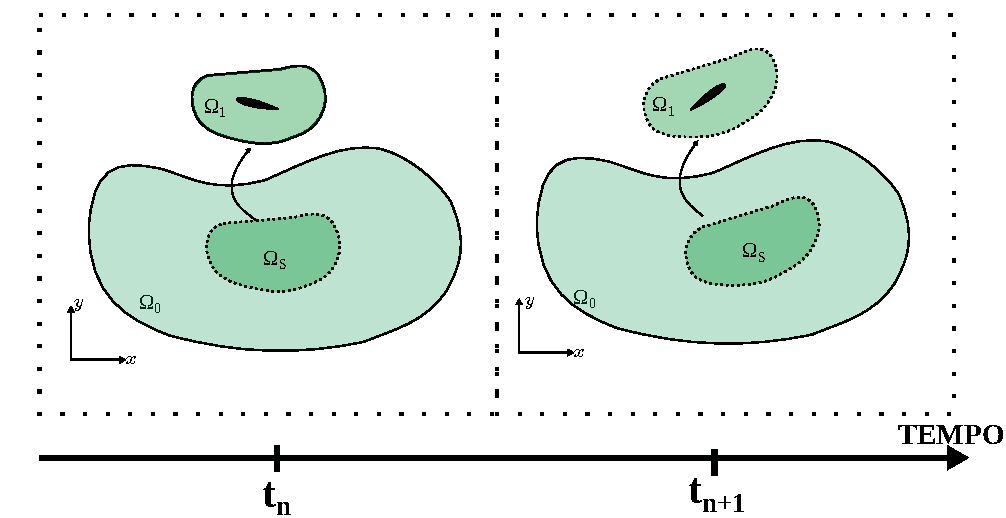
\includegraphics[scale=1.0,trim=0cm 0cm 0cm 0cm, clip=true]{Imagens/Cap6/dominioArlequinMoving.pdf}}	
	\caption{Domínio Arlequin móvel}
	\label{fig:ArlquinMóvel}
\end{figure}


\section{Implementação Computacional}

\section{Exemplos}

\subsection{Escoamento sobre um aerofólio NACA 0012}


\begin{figure}[htb!]
	\centering 
	{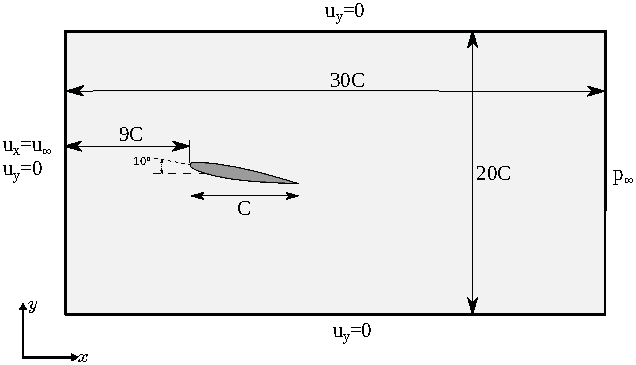
\includegraphics[scale=1.0,trim=0cm 0cm 0cm 0cm, clip=true]{Imagens/Cap6/aerofolio.pdf}}	
	\caption{Geometria Aerofólio}
	\label{fig:Aerofolio}
\end{figure}



\begin{figure}[htb!]
	\centering 
	{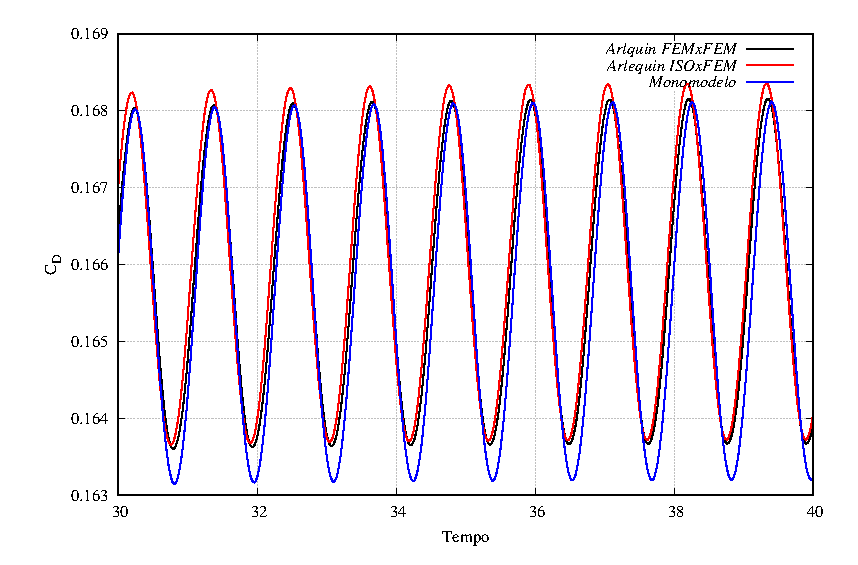
\includegraphics[scale=1.0,trim=0cm 0cm 0cm 0cm, clip=true]{Imagens/Cap6/DragRe.eps}}	
	\caption{Coeficiente de Arrasto}
	\label{fig:AeroDrag}
\end{figure}



\begin{figure}[htb!]
	\centering 
	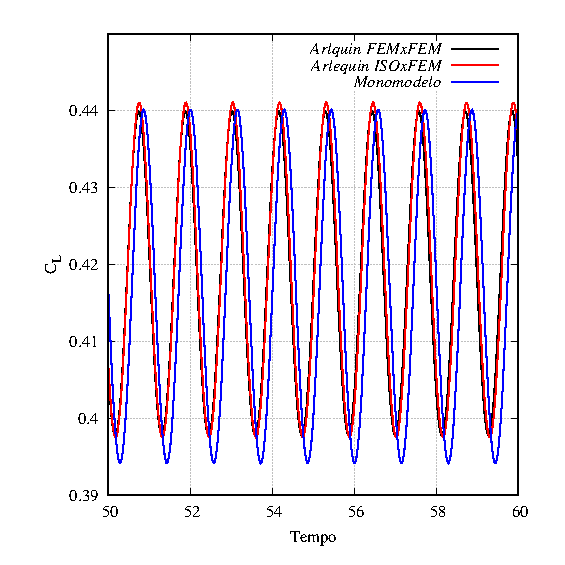
\includegraphics[scale=1.0,trim=0cm 0cm 0cm 0cm, clip=true]{Imagens/Cap6/LiftRe.eps}	
	\caption{Coeficiente de Sustentação}
	\label{fig:AeroLift}
\end{figure}



\subsection{Aerofólio com movimento de arfagem prescrito}


\begin{figure}[htb!]
	\centering 
	{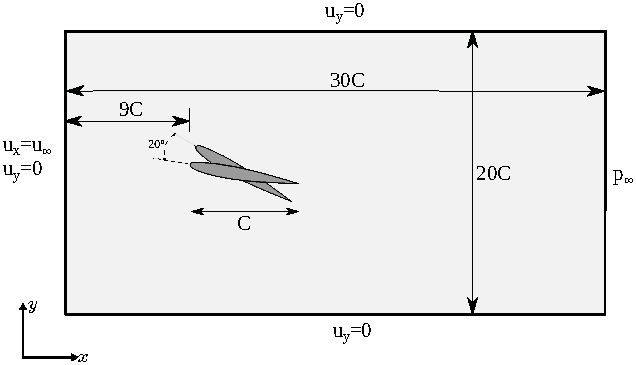
\includegraphics[scale=1.0,trim=0cm 0cm 0cm 0cm, clip=true]{Imagens/Cap6/aerofolioMov.pdf}}	
	\caption{Geometria Aerofólio}
	\label{fig:AerofolioMoving}
\end{figure}



\begin{figure}[htb!]
	\centering 
	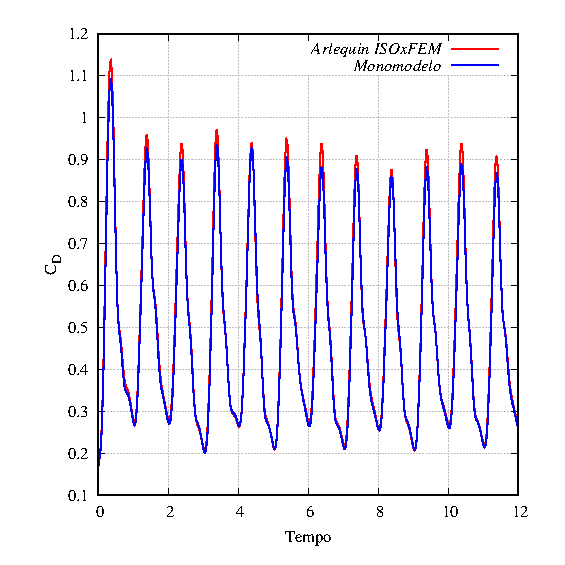
\includegraphics[scale=1.0,trim=0cm 0cm 0cm 0cm, clip=true]{Imagens/Cap6/DragMov.eps}	
	\caption{Coeficiente de Arrasto}
	\label{fig:AeroDragMov}
\end{figure}

\begin{figure}[htb!]
	\centering 
	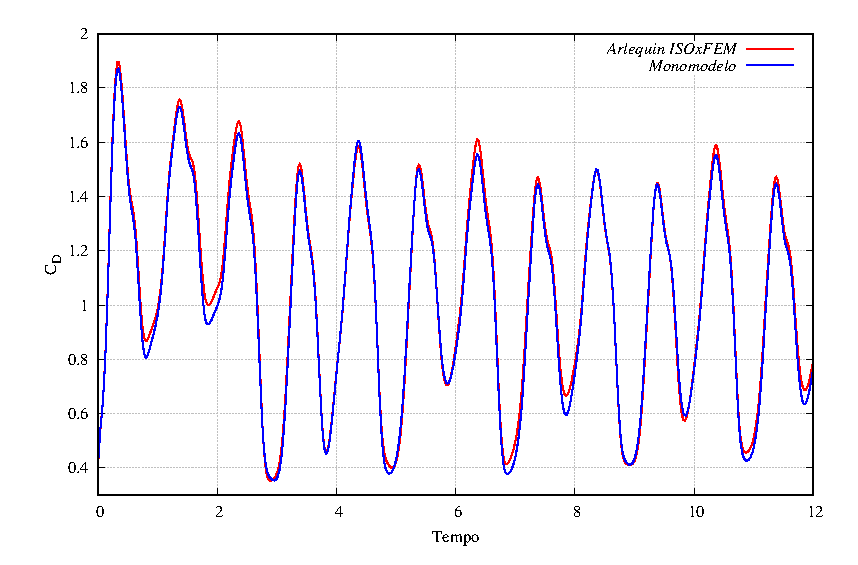
\includegraphics[scale=1.0,trim=0cm 0cm 0cm 0cm, clip=true]{Imagens/Cap6/LiftMov.eps}	
	\caption{Coeficiente de Sustentação}
	\label{fig:AeroLiftMov}
\end{figure}

\end{document}
